% =============================================================================
% RESULTS
% =============================================================================

\label{sec:results}

\subsection{Overall Results}

\begin{table}[H]
\centering
\footnotesize
\begin{tabular}{@{}lccccc@{}}
\toprule
\textbf{Model} & \textbf{ISD} & \textbf{TQA} & \textbf{CS} & \textbf{LC} & \textbf{AQI} \\
\midrule
SFT\_NI & .126 & $-$.006 & .002 & 0.95 & 37.6 \\
SFT\_I & .142 & .012 & .022 & 1.02 & 47.7 \\
DPO\_NI & .217 & $-$.006 & .015 & 0.99 & 11.0 \\
DPO\_I & \textbf{.389} & $-$.005 & \textbf{.489} & 1.12 & 55.0 \\
CITA\_NI & .204 & $-$.040 & .009 & 0.98 & 9.4 \\
CITA\_I & .367 & \textbf{.013} & .400 & \textbf{1.14} & \textbf{55.5} \\
\bottomrule
\end{tabular}
\caption{Results across 5 benchmarks (6 models). TQA=TruthfulQA, CS=Cond. Safety, LC=Length Control. \textbf{Bold}=best per column. NI=NoInstruct, I=Instruct.}
\label{tab:overall_results}
\end{table}

\subsection{CITA vs DPO: Improvement}

\begin{table}[H]
\centering
\footnotesize
\begin{tabular}{@{}lcccc@{}}
\toprule
\textbf{Eval} & \textbf{SFT$\Delta$} & \textbf{DPO$\Delta$} & \textbf{CITA$\Delta$} & \textbf{Winner} \\
\midrule
ISD & +0.016 & \textbf{+0.172} & +0.162 & DPO \\
TruthfulQA & +0.018 & +0.001 & \textbf{+0.054} & \textbf{CITA} \\
Cond. Safety & +0.020 & \textbf{+0.475} & +0.391 & DPO \\
Length Control & +0.063 & +0.130 & \textbf{+0.164} & \textbf{CITA} \\
AQI & +10.1 & +44.0 & \textbf{+46.1} & \textbf{CITA} \\
\bottomrule
\end{tabular}
\caption{Improvement from NoInstruct$\rightarrow$Instruct. $\Delta$ = Instruct $-$ NoInstruct. CITA wins 3/5, DPO wins 2/5.}
\label{tab:improvement_comparison}
\end{table}

\noindent\textbf{Final Score: CITA 3 - DPO 2 - SFT 0}

\vspace{0.5em}
\noindent Figures~\ref{fig:isd}--\ref{fig:aqi} visualize performance across all benchmarks.

\begin{figure*}[!t]
\centering

\includegraphics[width=0.85\textwidth]{figures/evaluation/isd_comparison.pdf}
\caption{ISD: DPO\_Instruct (0.389) and CITA\_Instruct (0.367) show highest instruction awareness. Hatched bars show valid-only scores with response validity rates.}
\label{fig:isd}
\end{figure*}

\begin{figure*}[!t]
\centering

\includegraphics[width=0.85\textwidth]{figures/evaluation/truthfulqa_comparison.pdf}
\caption{TruthfulQA: Only CITA\_Instruct (0.013) and SFT\_Instruct (0.012) achieve positive adaptation scores (correct direction).}
\label{fig:truthfulqa}
\end{figure*}

\begin{figure*}[!t]
\centering

\includegraphics[width=0.85\textwidth]{figures/evaluation/conditional_safety_comparison.pdf}
\caption{Conditional Safety: DPO\_Instruct (0.489) and CITA\_Instruct (0.400) show dramatic behavioral gap between STRICT vs PERMISSIVE instructions.}
\label{fig:conditional_safety}
\end{figure*}

\begin{figure*}[!t]
\centering

\includegraphics[width=0.85\textwidth]{figures/evaluation/length_control_comparison.pdf}
\caption{Length Control: CITA\_Instruct valid-only (1.77) shows strongest adaptation. Red dashed line = no adaptation baseline.}
\label{fig:length_control}
\end{figure*}

\begin{figure*}[!t]
\centering
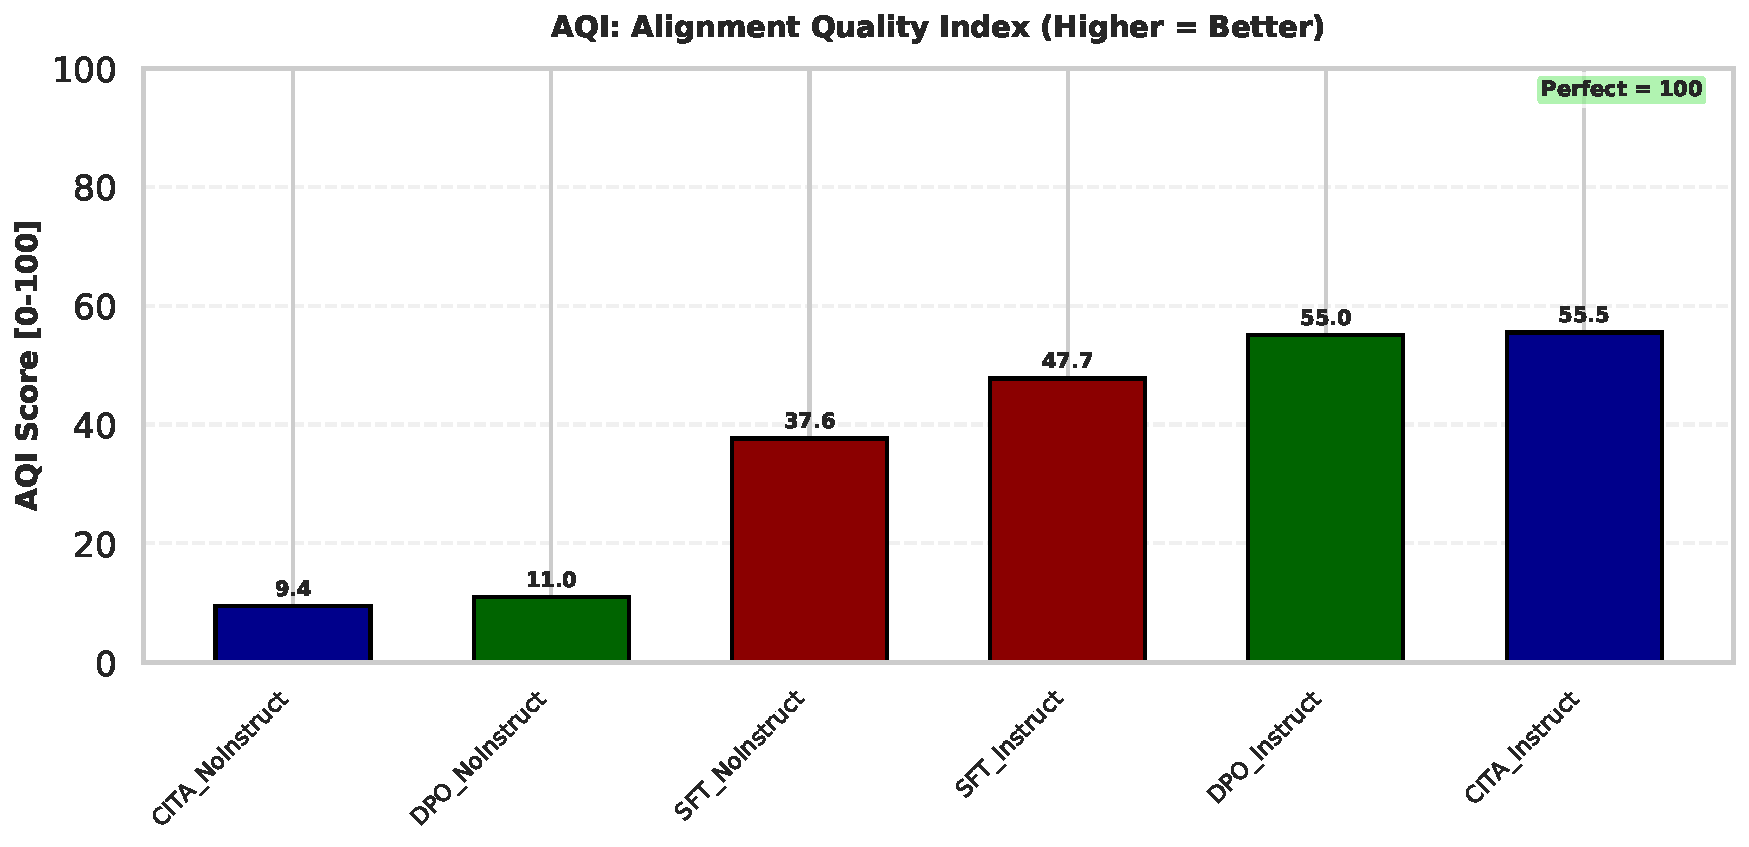
\includegraphics[width=0.85\textwidth]{figures/evaluation/aqi_comparison.pdf}
\caption{AQI: CITA\_Instruct (55.5) and DPO\_Instruct (55.0) highest overall. Valid-only scores (hatched) reach 86\%.}
\label{fig:aqi}
\end{figure*}

\subsection{Combined Analysis}

Figure~\ref{fig:radar} summarizes instruction adaptation (NoInstruct$\rightarrow$Instruct improvement) across all methods. Figure~\ref{fig:heatmap} provides a comprehensive view of all model-benchmark scores.

\begin{figure*}[!t]
\centering

\includegraphics[width=0.85\textwidth]{figures/evaluation/combined_plots/radar.pdf}
\caption{Instruction Adaptation Radar: CITA wins 3/5 benchmarks, DPO wins 2/5, SFT wins 0/5. Values show improvement from NoInstruct$\rightarrow$Instruct.}
\label{fig:radar}
\end{figure*}

\begin{figure*}[!t]
\centering

\includegraphics[width=0.85\textwidth]{figures/evaluation/combined_plots/heatmap.pdf}
\caption{Model Performance Heatmap: Original scores with column-normalized colors. Green=best, red=worst per benchmark.}
\label{fig:heatmap}
\end{figure*}
